\section{Methodology}
\label{sec:methodology}
% \subsection{Description}
% The methodology section explains your experimental setup.
% It should state every bit of information that is necessary in
% order to be able to reproduce your results. It further covers
% your actions taken in order to ensure that you are really
% measuring what you think you are measuring as well as your
% actions that were taken in order to validate your results. The
% goals are to set up realistic experiments and be absolutely
% convinced that you took care of all side-effects as well as to
% state enough information such that your experiments are fully
% reproducible.


To demonstrate the viability of a SSNN as a readout-layer in a RC-system, a simple software simulation was implemented in the Python programming language.
The implementation consists of three modules; a one-dimensional, homogenous, binary CA, an SSNN implementation and a genetic algorithm.
Figure shows how the CA and the SSNN is connected.

\begin{figure}
  \centering
  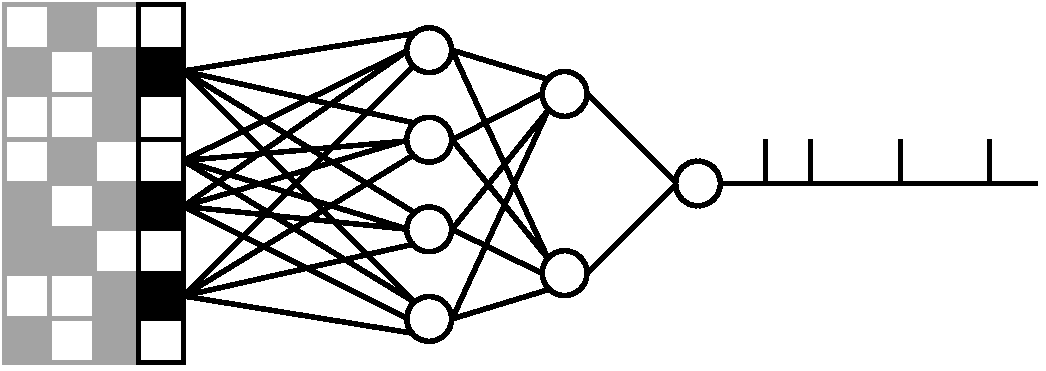
\includegraphics[width=\linewidth]{figures/rc-flow}
  \caption{At each timestep, the state of the CA is fed to the input-layer of the SSNN, which propagates updates through the network layers in a pipelined fashion.}
\label{fig:rc-flow}
\end{figure}

\subsection{Cellular Automata Module}

The CA consists of an array of 0s and 1s, and a step function that, given a CA-array, performs a single development step on it.
As the CA is homogenous, the same development rule, stored in a look-up-table, is applied to each cell every development step.
Since the state of the CA is stored in such a simple format, perturbing the system with input is as simple as replacing the array as a whole or modifying parts of it betweeen development steps.

\subsection{SSNN Readout Module}

\subsection{Genetic Algorithm}
